%%%%%%%%%%%%%%%%%%%%%%%%%%%%%%%%%%%%%%%%%
% Journal Article
% LaTeX Template
% Version 1.4 (15/5/16)
%
% This template has been downloaded from:
% http://www.LaTeXTemplates.com
%
% Original author:
% Frits Wenneker (http://www.howtotex.com) with extensive modifications by
% Vel (vel@LaTeXTemplates.com)
%
% License:
% CC BY-NC-SA 3.0 (http://creativecommons.org/licenses/by-nc-sa/3.0/)
%
%%%%%%%%%%%%%%%%%%%%%%%%%%%%%%%%%%%%%%%%%

%----------------------------------------------------------------------------------------
%	PACKAGES AND OTHER DOCUMENT CONFIGURATIONS
%----------------------------------------------------------------------------------------

\documentclass[10pt]{article} % Single column

%\documentclass[twoside,twocolumn]{article} % Two column

\usepackage{blindtext} % Package to generate dummy text throughout this template 

\usepackage[sc]{mathpazo} % Use the Palatino font
\usepackage[T1]{fontenc} % Use 8-bit encoding that has 256 glyphs
\linespread{1.05} % Line spacing - Palatino needs more space between lines
\usepackage{microtype} % Slightly tweak font spacing for aesthetics

\usepackage[spanish]{babel} % Language hyphenation and typographical rules

\usepackage[hmarginratio=1:1,top=32mm,columnsep=20pt]{geometry} % Document margins
\usepackage[hang, small,labelfont=bf,up,textfont=it,up]{caption} % Custom captions under/above floats in tables or figures
\usepackage{booktabs} % Horizontal rules in tables

\usepackage{lettrine} % The lettrine is the first enlarged letter at the beginning of the text

\usepackage{enumitem} % Customized lists
\setlist[itemize]{noitemsep} % Make itemize lists more compact

\usepackage{abstract} % Allows abstract customization
\renewcommand{\abstractnamefont}{\normalfont\bfseries} % Set the "Abstract" text to bold
\renewcommand{\abstracttextfont}{\normalfont\small\itshape} % Set the abstract itself to small italic text

\usepackage{titlesec} % Allows customization of titles
\renewcommand\thesection{\Roman{section}} % Roman numerals for the sections
\renewcommand\thesubsection{\roman{subsection}} % roman numerals for subsections
\titleformat{\section}[block]{\large\scshape\centering}{\thesection.}{1em}{} % Change the look of the section titles
\titleformat{\subsection}[block]{\large}{\thesubsection.}{1em}{} % Change the look of the section titles

\usepackage{fancyhdr} % Headers and footers
\pagestyle{fancy} % All pages have headers and footers
\fancyhead{} % Blank out the default header
\fancyfoot{} % Blank out the default footer
\fancyhead[C]{Dise\~no y An\'alisis de Algoritmos. \textbf{Proyecto \# 2: Tito el corrupto}} % Custom header text
\fancyfoot[RO,LE]{\thepage} % Custom footer text

\usepackage{titling} % Customizing the title section

\usepackage{hyperref} % For hyperlinks in the PDF

\usepackage{graphicx} % For images

\usepackage{pifont} % bullets

\usepackage{amsmath}

\usepackage{algpseudocode}

% Keywords command
\providecommand{\keywords}[1]
{
	\small	
	\vspace{0.5em}
	\noindent \textbf{\textit{Palabras clave --- }} #1
}


%----------------------------------------------------------------------------------------
%	TITLE SECTION
%----------------------------------------------------------------------------------------

\setlength{\droptitle}{-4\baselineskip} % Move the title up

\pretitle{\begin{center}\Huge\bfseries} % Article title formatting
	\posttitle{\end{center}} % Article title closing formatting
\title{\normalsize{Dise\~no y An\'alisis de Algoritmos }\\
	\Huge\bfseries Proyecto \# 2: Tito el corrupto \\
} % Article title
\author{% 
	%
\includegraphics[width=15em]{logo.png}\\
	Laura Victoria Riera P\'erez\\
	Mari\'e del Valle Reyes \vspace{1em} \\
	\small Cuarto a\~no. Ciencias de la Computaci\'on. \\ % institution
	\small Facultad de Matem\'atica y Computaci\'on, Universidad de La Habana, Cuba \\ % institution
}
\date{\footnotesize \today } % Leave empty to omit a date


% Abstract configurations
\renewenvironment{abstract}
{\small
	\begin{center}
		\bfseries \abstractname\vspace{-.5em}\vspace{0pt}
	\end{center}
	\list{}{
		\setlength{\leftmargin}{1.5cm}%
		\setlength{\rightmargin}{\leftmargin}%
	}%
	\item\relax}
{\endlist}

\usepackage{amsthm}
\usepackage{amssymb}
\usepackage{todonotes} % \TODO
\usepackage{listings} % Code listings
\usepackage{xcolor}

\definecolor{backcolour}{rgb}{0.95,0.95,0.92}

\newcommand{\csl}[1]{\colorbox{backcolour}{\texttt{#1}}}

\newcommand{\imgcaption}[2]{\tiny \textbf{Figura #1.} #2.}

\newcommand{\mgc}[2][]{\colorbox{backcolour}{\texttt{\_\_#2\_\_#1}}}

\newcommand{\mgccapt}[1]{\texttt{\_\_#1\_\_}}

\newtheorem{thm}{Teorema}
\newtheorem{mydef}{Definici\'on}%[section]
\newtheorem{lem}{Lema}
\newtheorem{fig}{\scriptsize{Figura}}


\renewcommand{\qedsymbol}{\rule{0.7em}{0.7em}}

% Hyperlinks configurations
\hypersetup{
	colorlinks=true,
	linkcolor=black,
	filecolor=magenta,      
	urlcolor=cyan,
	pdftitle={Overleaf Example},
	pdfpagemode=FullScreen,
}

%----------------------------------------------------------------------------------------

\begin{document}
	% Print the title
	\maketitle
	
	%----------------------------------------------------------------------------------------
	%	ARTICLE CONTENTS
	%----------------------------------------------------------------------------------------
	
	\section{Repositorio del proyecto}
	
	\begin{center}
		\href{https://github.com/computer-science-crows/algorithms-design-and-analysis}{https://github.com/computer-science-crows/algorithms-design-and-analysis}
	\end{center}

	\section{Definici\'on inicial del problema} 
	
	Tito se dió cuenta de que la carrera de computación estaba acabando con él y un día decidió darle un cambio radical a su vida. Comenzó a estudiar Ingeniería Industrial. Luego de unos años de fiesta, logró finalmente conseguir su título de ingeniero. Luego de otros tantos años ejerciendo sus estudios (¿?), consiguió ponerse a la cabeza de un gran proyecto de construcción de carreteras.
	
	La zona en la que debe trabajar tiene $n$ ciudades con $m$ posibles carreteras a construir entre ellas. 
	
	Cada ciudad que sea incluida en el proyecto aportará $a_i$ dólares al proyecto, mientras que cada carretera tiene un costo de $w_i$ dólares. 
	
	Si una carretera se incluye en el proyecto, las ciudades unidas por esta también deben incluirse.
	
	El problema está en que Tito quiere utilizar una de las habilidades que aprendió en sus años de estudio, la de la malversación de fondos. 
	
	Todo el dinero necesario para el proyecto que no sea un aporte de alguna ciudad, lo proveerá el país y pasará por manos de Tito. 
	
	El dinero aportado por las ciudades no pasará por sus manos. 
	
	Tito quiere maximizar la cantidad de dinero que pasa por él, para poder hacer su magia. Ayude a Tito a seleccionar el conjunto de carreteras a incluir en el proyecto para lograr su objetivo.
	
	\section{Definici\'on en t\'erminos matem\'atico - computacionales}
	
	\subsection{Preliminares}
	
	\section{L\'inea de pensamiento}
	
	\section{Algoritmo}
	
	\subsection{Explicaci\'on del algoritmo}
	
	\subsection{Complejidad Temporal}
	
	\subsection{Complejidad espacial}
		
	\section{Generador de casos de prueba}
	
	En \textit{src/app/generator.py} fue implementado un generador, el cual recibe una cantidad $ s $ de muestras a producir, genera valores random con el formato de entrada de los algoritmos implementados, halla la soluci\'on \'optima con $ backtrack $ y las guarda en $ json/test\_cases.json $. Se generaron 3000 casos de prueba, con $ n $ m\'aximo igual a 11, dado que, como se mencion\'o anteriormente, es lo que puede ejecutar el $ backtrack $.
	
	\section{Tester}
	En \textit{src/app/tester.py} fue implementado un tester, que recibe una funci\'on y prueba el desempe\~no de la misma en cuanto a si obtuvo la soluci\'on \'optima o no, y el tiempo que demor\'o en hacerlo, comparando con los casos de prueba obtenidos con el generador. Dichos resultados se muestran en consola de la siguiente forma:
%		 \begin{center}
%	 		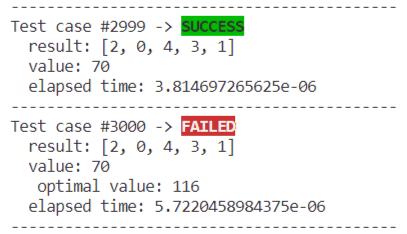
\includegraphics[width=7cm]{tester_sample.png}
%	 		
%	 		\tiny{\textbf{Figura 1.} Ejemplo de c\'omo se muestran los tests de una funci\'on en consola.} 
%	 	\end{center}
	 
	 Adem\'as, estos resultados se guardan en un $ .json $ con el nombre de la funci\'on en la carpeta tests. Las soluciones implementadas fueron testeadas para todos los casos de prueba generados y pueden encontrarse en $ json/tests/simplex\_solution.json $ y $ json/tests/hungarian\_solution.json $
	
	\section{Comparaci\'on de soluciones implementadas}
	
	\begin{thebibliography}
		a
		\bibitem{introduction} Cormen, Thomas H. y otros. \emph{Introduction to Algorithms}. 
		The MIT Press.
		4ta Edici\'on.		
		Cambridge, Massachusetts.
		2022.
	\end{thebibliography}
\end{document}


